% !TeX root=../main.tex
\chapter{پیاده سازی رویکرد مبتنی بر گراف جهت مکان‌یابی و کالیبراسیون همزمان برای ربات‌های کابلی صلب}

در فصل قبل رویکردی بر مبنای ساختار گراف برای انجام مسئله کالیبراسیون و مکان‌یابی ربات به صورت زمان واقعی ارائه شد. ویژگی‌هایی برای این رویکرد ارائه شد که حل این مسئله پیچیده و پرکاربرد رباتیکی را تسهیل کرده و باعث بهبود نتایج بهینه‌سازی شده است. در این فصل پیاده‌سازی کاملی از گراف‌های معرفی شده بر روی یک ربات خواهیم داشت. سعی بر آن بوده که ربات انتخاب شده برای این پیاده‌سازی از نظر سینماتیک و دینامیک دارای معادلاتی نسبتاً پیچیده باشد تا قدرت و سرعت این الگوریتم را مورد بررسی کافی قرار دهیم.


\section{انتخاب ربات مناسب جهت توسعه الگوریتم}

ربات نمونه انتخاب شده برای ارائه این فرمول‌بندی، یک ربات چهار کابلی فروتحریک آسان نصب می‌باشد. علت انتخاب این نوع ربات آسان نصب به عنوان موضوع مورد بررسی، قابلیت استفاده زیاد آنها در کارکردهای متنوع رباتیکی می‌باشد، به شرطی که هر بار پس از نصب در هر محیط دلخواه فرآیند کالیبراسیون بدون زمان‌بر و با کمترین زحمت انجام شود. فرمول‌بندی انجام شده برای این ربات به نحوی است که منجر به یک کالیبراسیون خودکار در کنار مکان‌یابی تنها با همان حسگرهایی که در ربات برای مکان‌یابی تعبیه شده است، بدون زحمت اضافی برای کاربر انجام می‌شود. نتیجه این رویکرد علاوه بر افزایش دقت نهایی این فرآیندها، مفهومی حقیقی‌تر به آسان نصب بودن به این دسته از ربات‌های کابلی می‌بخشد.

آنچه تا کنون بیشتر مورد بررسی قرار گرفته حل مسئله کالیبراسیون برای ربات‌هایی است که کابل آنها به عنوان جسمی صلب در نظر گرفته می‌شود. این فرض اساسی حل مسئله را آسان‌تر می‌کند. در ادامه‌ی این فصل ما با استفاده از رویکرد بیان شده، کالیبراسیون و مکان‌یابی را برای یک ربات کابلی با فرض یاد شده انجام می‌دهیم و نتایج را مورد بررسی قرار می‌دهیم. علی‌رغم اینکه این فرض حل مسئله را ساده‌تر می‌کند، زمانی که نسبت جرم پنجه ربات به جرم کابل‌ها زیاد شود، این فرض قابل قبول نخواهد بود. نشان خواهیم داد که با افزایش این میزان شکم‌دهی که معمولاً در ربات‌هایی با ابعاد بزرگتر دیده می‌شود، کالیبراسیون و مکان‌یابی با مشکل مواجه خواهد شد. راه حل ارائه شده برای حل این مشکل، ایجاد مسئله‌ای شامل قیدهای دینامیکی پیچیده کابل ها هستند. در این فصل سعی بر ایجاد گرافی خواهیم‌داشت که مسئله تعریف شده برای ربات کابلی صلب را حل کند. در فصل بعد، با مقید‌سازی این گراف، مسئله‌ای کامل‌تر  را فرمول‌بندی خواهیم کرد که مشکل مطرح شده را نیز آدرس‌دهی کند.


\section{توسعه گراف عامل برای یک ربات چهار کابلی با فرض کابل صلب}
در این بخش، انجام فرآیند کالیبراسیون و مکان‌یابی به صورت همزمان برای یک ربات کابلی با در نظر گرفتن فرض صلب بودن کابل‌ها با رویکرد گراف-مبنا انجام می‌شود. برای این فرآیند، ابتدا ربات چهار کابلی ARASCam معرفی می‌گردد. سپس فرضیاتی بر روی ساختار ربات ایجاد شده و با در نظر گرفتن این فرضیات، فرمول‌بندی جامعی برای ربات ارائه می‌شود. در نهایت، از این فرمول‌بندی برای پیاده‌سازی گراف عامل معرفی شده استفاده می‌شود و نتایج مورد بررسی قرار می‌گیرد. 

\subsection{معرفی ربات کابلی ARASCam}
ربات \lr{ARASCam} که در گروه تحقیقاتی رباتیک \lr{ARAS} توسعه یافته است، یک ربات معلق فروتحریک موازی با کابل‌های محرک و با شش درجه آزادی می‌باشد. شکل 
\ref{fig:arascam}
 نسخه اولیه این  ربات که برای یک فضای کاری نسبتا کوچک آزمایشگاهی طراحی شده است را نشان می دهد. همانطور که در تصویر مشاهده می شود، پنجه ربات که مجهز به یک دوبین تعبیه شده بر روی پردازنده 
\lr{Raspberry PI} 
می باشد، توسط چهار کابل در فضا معلق شده است. $\boldsymbol{B}$ بیانگر دستگاه مختصات پایه و همچنین $\boldsymbol{E}$ نشاه دهنده دستگاه مختصات پنجه ربات می باشد. $i$ امین کابل در نقطه ${}^B\!\boldsymbol{b}_i$ در مختصات پنجه به ربات و در نقطه ${}^E\!\boldsymbol{a}_i$ در مختصات پایه به پولی متناظر آن متصل می شود. ماتریس انتقال از دستگاه مختصات پایه به پنجه با 
$\boldsymbol{T}^{\boldsymbol{B}}_{\boldsymbol{E}}$
نشان داده شده است.


در این ربات، کابل‌ها با استفاده از یک سیستم مکانیکی درام جمع و باز می‌شوند. هر یک از کابل‌ها پس از خروج از درام، توسط مکانیزم مکانیکی از روی سنسور نیرو عبور کرده و سپس به پولی منتقل می‌شود. در نهایت، از نقطه مشخصی در پولی به ربات متصل می‌شود. همچنین از آنجایی که در این ربات نسبت جرم پنجه به جرم کابل‌های ربات مقدار زیادی است، می توان از شکم‌دهی کابل های آن صرف نظر کرد و کابل های آن را به عنوان اجسام صلب مدل کرد.

\begin{figure}
	\centering
	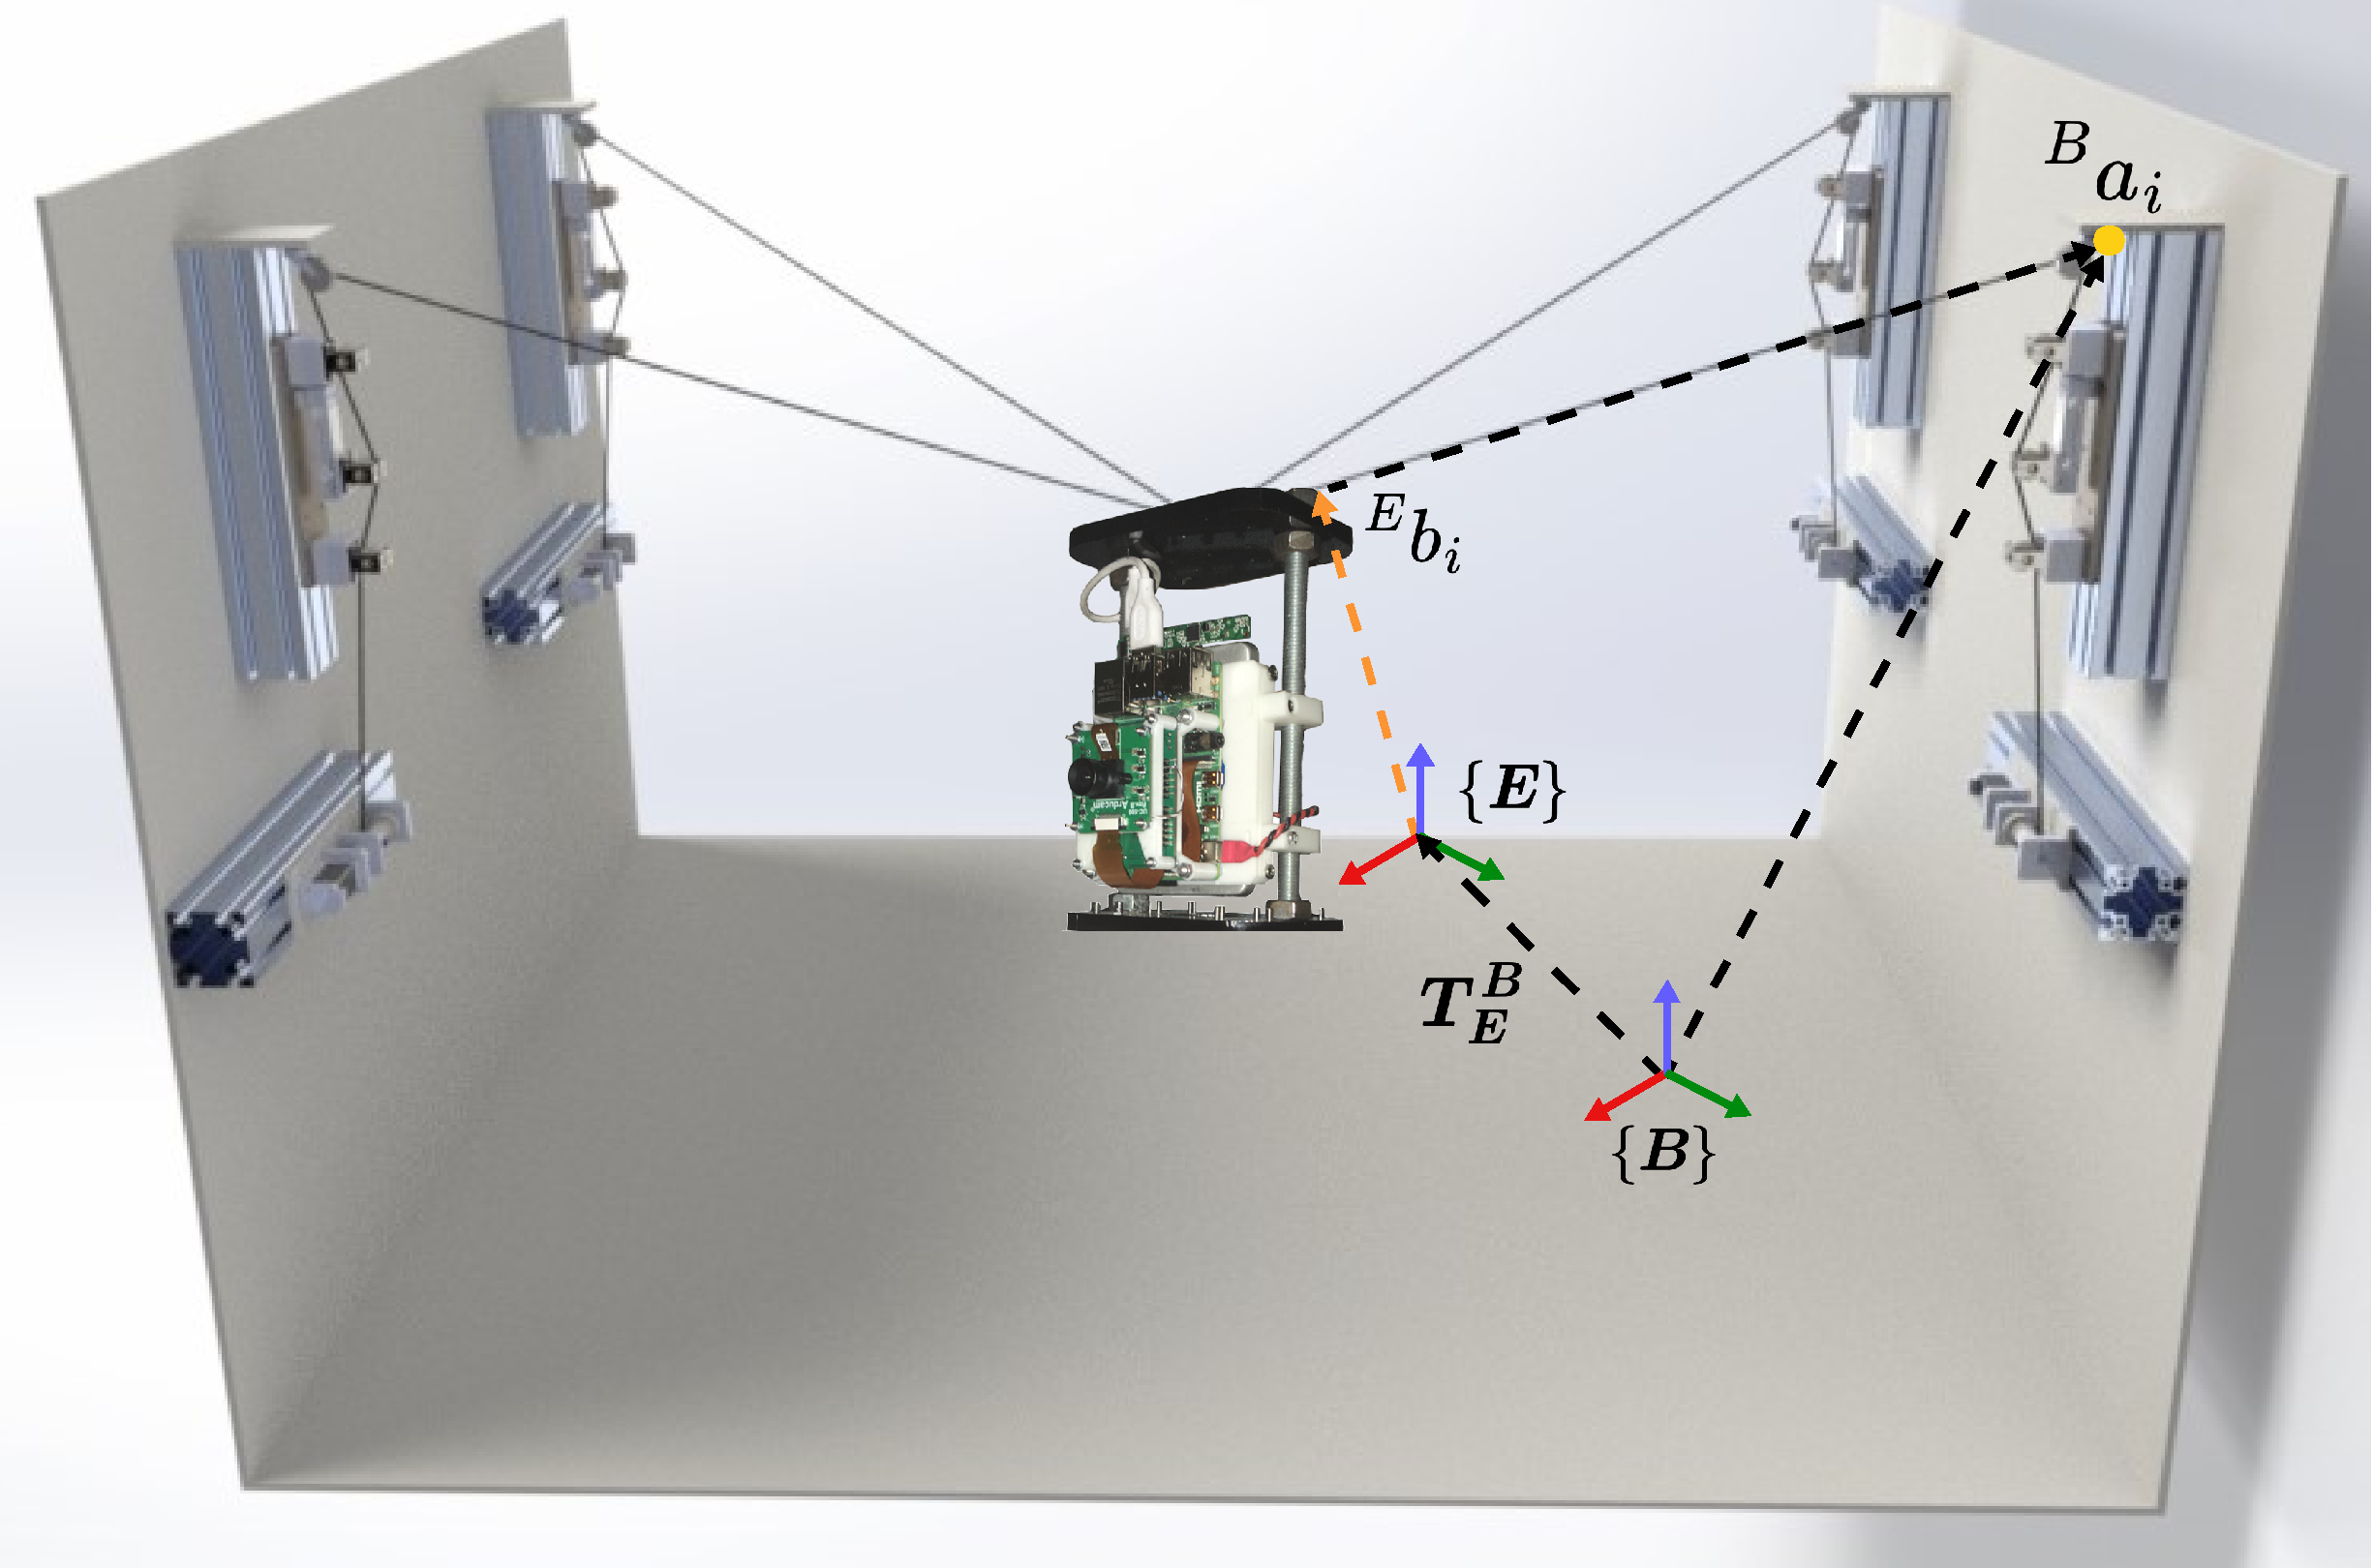
\includegraphics[width=0.5\linewidth]{img/arascam}
	\caption{نمایی از ربات چهار کابلی فروتحریک معلق ARAS-CAM}
	\label{fig:arascam}
\end{figure}

\subsection{بیان فرمول‌بندی مسئله و فرضیات} \label{seq:formulation_rigid}
برای فرمول‌بندی مسئله از هندسه بیان شده در شکل 
\ref{fig:arascam}
استفاده می کنیم. برای یک ربات با کابل‌های صلب، مدل اندازه‌گیری طول کابل \( \hat{z}_i \) با استفاده از حسگر انکودر روی ربات برای نمونه $k$، به صورت زیر می تواند فرمول‌بندی ‌شود:
\begin{equation}\label{eq:cable_length_without_young_module}
	\begin{split}
		l^\star_i [k] &\triangleq \| \boldsymbol{R}^B_E ~ {}^B\!\boldsymbol{b}_i + {}^B\!\boldsymbol{t}_E^B - {}^B\!\boldsymbol{a}_i \|^2 \\
		\hat{z}_i [k] &= l^\star_i [k] + l_{i}^0 + w_{\text{enc}} [k]
	\end{split}
\end{equation}


که در آن
\( (\boldsymbol{R}^B_E, {}^B\!\boldsymbol{t}_E^B) \)
 نشان‌دهنده ماتریس جهت‌گیری و بردار انتقال پنجه در دستگاه مختصات پایه،
\(l_{i}^0  \)
نشان‌دهنده مقدار جابجایی اولیه انکودر، و 
\( w_{\text{enc}} [k] \)
 نشان‌دهنده نویز اندازه‌گیری طول است. اگر انعطاف‌پذیری کابل نیز در نظر گرفته شود، نیروی
\( T_i \)
 در کابل، طول اندازه‌گیری شده کابل را به صورت زیر تغییر می‌دهد:
\begin{equation} \label{eq:cable_length_with_young_module}
	\hat{z}_i [k] = \left(1 - \frac{T_i [k] + w_T [k]}{EA} \right) l^\star_i [k] + l_{i}^0 + w_{\text{enc}} [k]
\end{equation}


که در آن \( E \) مدول یانگ کابل، \( A \) سطح مقطع کابل، و \( w_T [k] \) نویز اندازه‌گیری نیرو است. چنانچه نیروی کابل صفر باشد،
\( T_i [k] = 0 \)، 
در معادله 
\ref{eq:cable_length_with_young_module}
 طول اندازه‌گیری شده توسط انکودر با فاصله واقعی بین \( a_i \) و \( b_i \) مطابقت دارد. با این حال، در پیکربندی‌ای که موتور در محل قفل شده و انکودر مقدار ثابتی را می‌خواند، جابجایی طول به دلیل کشیدگی توسط انکودر دیده نمی‌شود اما نسخه مقیاس‌شده وابسته به نیرو از فاصله واقعی \( l^\star_i [k] \) اندازه‌گیری می‌شود. با افزایش \( E \) (کابل‌های سفت)، اهمیت این مقیاس‌بندی وابسته به نیرو به صفر کاهش می‌یابد و معادله 
\ref{eq:cable_length_with_young_module}
به معادله
\ref{eq:cable_length_without_young_module}
 ساده می‌شود. در مورد ربات‌ با کابل‌های انعطاف‌پذیر، فرض می‌کنیم که حسگرهای نیروی کابل در نزدیکی عملگرها قرار گرفته‌اند. با این حال، برای بسیاری از کاربردها که به ربات‌های کابلی با اندازه متوسط نیاز دارند، انعطاف‌پذیری کابل ممکن است با انتخاب مناسب کابل‌ها قابل صرف نظر باشد.

علاوه بر فرمول‌بندی سینماتیک، مطابق شکل
\ref{fig:arascam}
 ربات با یک دوربین روی انتهای ربات، متصل به پنجه، تجهیز شده است. در اینجا ما تصاویر دریافتی از این دوربین را با استفاده از الگوریتم SVO
\cite{Forster2014ICRA}
  برای تولید اندازه‌گیری‌های مکان ربات در فضای
$SE(3)$
به سیستم وارد می کنیم که بدین‌ترتیب برای مکان‌یابی ربات زنجیره‌ای از تغیرات مسافت‌پیمایی با فرمول بندی زیر به هم وصل می‌شوند:
\begin{equation}
	\Delta \boldsymbol{T}^k_{k-1} = \begin{bmatrix} \boldsymbol{R}^k_{k-1} & \boldsymbol{t}^k_{k-1} \\ \boldsymbol{0} & s^{-1} \end{bmatrix}
\end{equation}

در طول مرحله کالیبراسیون و مکان‌یابی با استفاده از این الگوریتم، فرض می‌کنیم محیط‌ دارای نور خوب با بافت‌های غنی از ویژگی بوده و دوربین به آرامی حرکت می‌کند.  مسئله کالیبراسیون و مکان‌یابی به تخمین مشترک مکان‌های ربات
$\boldsymbol{T}^B_E [k]$,
مکان‌های نقاط اتصال کابل‌ها به پولی‌های متناظر
$\boldsymbol{a}_i$،
 طول‌های اولیه کابل‌ها
$l_{i}^0$،
و مقیاس الگوریتم مسافت‌پیمایی
$s$
با استفاده از اندازه‌گیری‌های الگوریتم مسافت‌پیمایی
 \( \Delta \boldsymbol{T}^k_{k-1} \)،
انکودرهای طول کابل
$z_i [k]$،
و برای ربات‌ها با کابل‌های انعطاف‌پذیر، اندازه‌گیری‌های نیرو 
$T_i$ 
کاهش می‌یابد. این تصویر از تخمین مشترک به حل یک مسئله بهینه‌سازی منجر می‌شود که مدل سینماتیکی را به اندازه‌گیری‌های انجام شده نزدیک‌تر کند. به عبارتی دیگر، فرمول‌بندی که در
 \ref{eq:optimization_equation_conventional_multi_sensor_measurement} 
 ایجاد شد، در اینجا به فرمول‌بندی زیر بازنویسی می‌شود:
\begin{equation}
	\min_{\boldsymbol{a}_i, l_{i}^0, \boldsymbol{T}^B_E [k], s} \sum_k \| h(\boldsymbol{a}_i, l_{i}^0, \boldsymbol{T}^B_E [k], s) - z_i [k] \|^2_2
\end{equation}

که مدل اندازه‌گیری، \( h(.) \)، به صورت زیر تعریف می‌شود:
\begin{equation} \label{eq:mathmatic_model_rigid_cable}
	h(\boldsymbol{a}_i, l_{i}^0, \boldsymbol{T}^B_E [k], s) = s \left( 1 - \frac{T_i [k] + w_T [k]}{EA} \right) l^\star_i [k] + l_{i}^0 + w_{\text{enc}} [k] 
\end{equation}
با این فرمول‌بندی، مقادیر بهینه نقاط پولی‌های ربات
$a_i^*$
و مکان‌های پنجه ربات
$\boldsymbol{t}^{B^{*}}_{E}$
با پارامتر بزرگنمایی
$s$
به دست می‌آید.


\subsection{رویت‌پذیری}
برای تحلیل مشاهده‌پذیری، از روش ارائه شده در
\cite{blueml2021bias}
الهام گرفته‌ایم که از سیستم‌های مکان‌یابی  UWB\footnote{\lr{Ultra Wide Band (UWB)}}
برای مقادیر اولیه الگوریتم بهینه‌سازی خود استفاده کرده‌است. با توجه به مدل اندازه‌گیری در معادله
\ref{eq:cable_length_with_young_module}
، می‌توان مسئله حداقل مربعات را به صورت خطی زیر بازنویسی کرد:
\begin{equation}\label{eq:observibility}
	\begin{bmatrix}
		-2t_x[1]\alpha[1] & \cdots & -2t_x[k]\alpha[k] \\
		-2t_y[1]\alpha[1] & \cdots & -2t_y[k]\alpha[k] \\
		-2t_z[1]\alpha[1] & \cdots & -2t_z[k]\alpha[k] \\
		d^2_t[1]\alpha[1] & \cdots & d^2_t[k]\alpha[k] \\
		2z_i[1] & \cdots & 2z_i[k] \\
		\alpha[1] & \cdots & \alpha[k]
	\end{bmatrix}^T
	\begin{bmatrix}
		s^2 a_x \\
		s^2 a_y \\
		s^2 a_z \\
		s^2 \\
		l_{0_i} \\
		s^2 (d^2_a - l_{0_i}^2)
	\end{bmatrix}
	=
	\begin{bmatrix}
		z_i[1]^2 \\
		z_i[2]^2 \\
		\vdots \\
		z_i[k]^2
	\end{bmatrix}
\end{equation}

که در آن \( d_a \)، \( d_t[k] \) و \( \alpha[k] \) به صورت زیر تعریف می‌شوند:
\begin{equation}
	\begin{split}
		\alpha[k] &\triangleq \left(1 - \frac{\tau_i[k]}{EA}\right) \\
		d^2_t[k] &\triangleq t^2_x[k] + t^2_y[k] + t^2_z[k], \quad d^2_a \triangleq t^2_x + a^2_y + a^2_z
	\end{split}
\end{equation}

همان‌طور که در 
\cite{blueml2021bias}
اشاره شده است، سیستم خطی در معادله 
\ref{eq:observibility}
معمولاً در عمل خوش تعریف\footnote{\lr{well-pose}}
و منجر به پاسخ‌های ضعیف خواهد شد. ما به جای این روش معرفی شده برای نقطه شروع، از چارچوب احتمالی استفاده می‌کنیم تا راه‌حل‌های با کیفیت بالاتری به دست آوریم. با این حال، وجود یک پاسخ برای این سیستم خطی، مشاهده‌پذیری پارامترهای سینماتیکی را با توجه به مجموعه اندازه‌گیری‌های تعریف شده در بخش قبلی اثبات می‌کند.









\section{بهینه‌سازی پارامترها با استفاده از گراف‌های عاملی} \label{seq:factor_graph_for_rigid_cable}

برای حل مسئله مکان‌یابی و کالیبراسیون ربات کابلی ارائه شده در شکل
\ref{fig:arascam}
در ساختار گراف، ما یک گراف عامل با گره‌های متغیر 
$\boldsymbol{X}(k) \in SE(3)$,
$l_{i}^0$,
$T_i(k), S \in \mathbb{R}$ 
و
$\boldsymbol{a}_i, \boldsymbol{b}_i(k) \in \mathbb{R}^3$ 
تعریف می‌کنیم که به ترتیب نمایانگر وضعیت دوربین، انحراف طول کابل (یا طول اولیه کابل)، نیرو‌های کابل، مکان نقاط پولی و نقاط اتصال کابل‌ها بر روی پنجه ربات هستند. شکل 
\ref{fig:rigidcable_factorgraph}
نشان‌دهنده این گراف می باشد. 
\begin{figure}
	\centering
	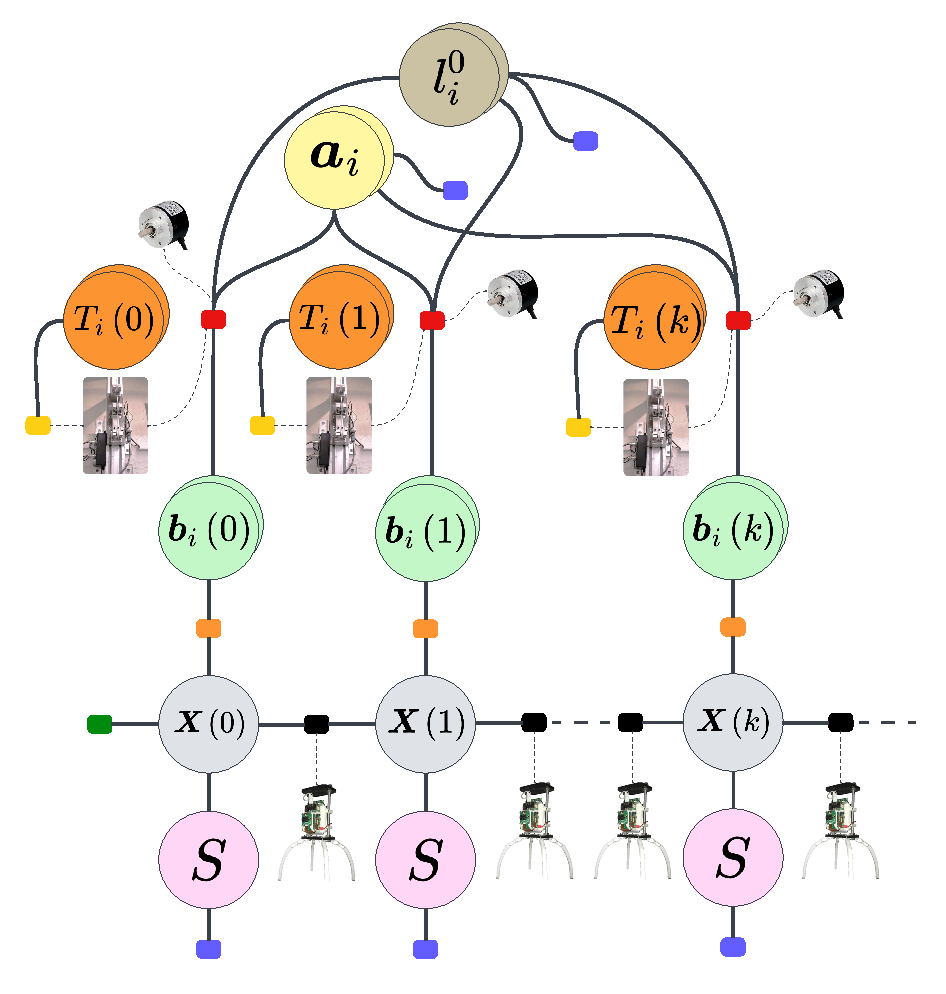
\includegraphics[width=0.6\linewidth]{img/rigidcable_factorgraph}
	\caption{گراف عامل پیشنهادی برای حل مسئله کالیبراسیون و مکان‌یابی ربات کابلی صلب}
	\label{fig:rigidcable_factorgraph}
\end{figure}


همانطور که در شکل 2 نشان داده شده است، گره‌های
$\boldsymbol{X}(k)$
با عامل‌های مسافت‌پیمایی مقیاس‌بندی شده (نشان داده شده با رنگ سیاه) که نشان‌دهنده مکان‌های نسبی و مقیاس‌دهی مسیر براساس مقدار گره مقیاس 
$S$
 است، به هم متصل می‌شوند. از سوی دیگر، هر وضعیت دوربین 
$\boldsymbol{X}(k)$
 به چهار نقطه اتصال کابل‌های در پنجه ربات
$\boldsymbol{b}_i(k)$
از طریق عامل‌های مکان نسبی (نشان داده شده با رنگ نارنجی) که با تبدیل‌های تعریف شده در مدل CAD پنجه ربات اولیه‌سازی شده‌اند، متصل می‌شود (که مشمول پارامترهای کالیبراسیون در این کار نیستند). هر یک از گره‌های
$\boldsymbol{b}_i(k)$
به نقاط اتصال پولی
$\boldsymbol{a}_i(k)$
از طریق عامل‌های سینماتیکی (نشان داده شده با رنگ قرمز) که طبق بخش 
\ref{seq:formulation_rigid}
 و با استفاده از مدل اندازه‌گیری
\ref{eq:mathmatic_model_rigid_cable}
تعریف شده‌اند، متصل می‌شوند.

همچنین، این عامل‌های سینماتیکی نیز به گره‌های نیروی کابل
$T_i(k)$
و پارامتر متغیر طول اولیه کابل
$l_{i}^0$
 متصل هستند. هر یک از این گره‌های نیرو کابل، توسط عامل‌های پیشین (نشان داده شده با رنگ زرد) با اندازه‌گیری‌های حسگر نیروسنج، محدود شده‌اند. همچنین، با استفاده از عامل پیشین متصل شده به اولین مکان پنجه ربات (نشان داده شده با رنگ سبز)، نقطه صفر مکان‌یابی ربات را می‌توان معین کرد. توجه داشته باشید که برای ربات‌های کابلی که کابل‌های با کیفیت بالا توسعه پیدا کرده‌اند، نیاز به اندازه‌گیری نیروی کابل ممکن است حذف شود و گره‌های
$T_i(k)$
از گراف عاملی حذف شوند. در این حالت، عوامل سینماتیکی باید براساس معادله
\ref{eq:cable_length_without_young_module}
تعریف شوند. 

در نهایت، با انتخاب مقادیر مناسبی برای میانگین و ماتریس‌های گوسی مقادیر اولیه عامل‌های متصل به گره‌های مقایس دهی (در بخش 
\ref{seq:monte_carlo}
روشی برای این انتخاب مناسب ارائه خواهد شد)، محل پولی‌ها و مقادیر اولیه طول کابل‌ها (نشان‌ داده شده با رنگ آبی) که به عنوان پارامترهای کالیبراسیون نقش بازی می کنند، گراف نهایی را تشکیل می‌دهیم. با استفاده از یک حل‌کننده مناسب می‌توان تابع بهینه‌ احتمالاتی نهایی را بهینه کرد. مقادیر گره‌های سینماتیکی بهینه شده و عدم قطعیت‌های به حاشیه رفته مربوطه خروجی نهایی چارچوب ما هستند.

\section{نتایج پیاده‌سازی}
این بخش به ارزیابی کاربردی بودن گراف پیشنهادی در تخمین مشترک پارامترهای سینماتیک و مکان‌های پنجه ربات، مستقل از دستگاه‌های اندازه‌گیری خارجی یا مقادیر اولیه پارامترها می‌پردازد. علاوه بر این، مزایای ترکیب بینایی-سینماتیک\footnote{\lr{Visual-Kinematic Fusion (VK-F)}}
 نیز در این بخش مورد بررسی قرار می‌گیرد.

\subsection{راه‌اندازی سیستم و فرضیات}
ما آزمایشات خود را با استفاده از ربات ARAS-CAM، یک ربات کابلی با اندازه متوسط و مساحت کاری 7 × 3 × 4 مترمکعب که توسط گروه رباتیک ARAS در دانشگاه صنعتی خواجه نصیرالدین طوسی توسعه داده شده است، انجام می‌دهیم.این ربات، به یک مجموعه کامل از حسگرهای سینماتیک و بینایی-اینرسی\footnote{\lr{Visual-Inertial (VI)}}
 مجهز شده است تا تحقیقات برآورد حالت برای ربات‌های کابلی را ممکن سازد. به طور خاص، هر واحد عملگر کابلی به یک حسگر نیرو با وضوح 
 $0.25$
  نیوتن و یک انکودر اندازه‌گیری طول نسبی با دقت 1 میلی‌متر مجهز شده است. از سوی دیگر، پنجه ربات دارای یک سیستم تعبیه شده با دوربین تک‌چشمی OV9281\footnote{\lr{monocular camera}}
 و واحد اندازه‌گیری اینرسی BMI088 است. برای پیش‌برد اهداف تحقیقات، 12 رشته داده با اندازه‌گیری‌های داده مرجع سه‌بعدی با استفاده از سیستم ردیابی مکانی توسعه یافته در این آزمایشگاه، از این ربات با عنوان مجموعه داده ARAS-CAM ضبط کرده‌ایم. برای پیاده‌سازی‌های انجام شده، ما از رشته داده 01 این مجموعه به عنوان نماینده حرکات پویاتر و از رشته داده 12 به عنوان یک همتای هموارتر استفاده می‌کنیم.

به دلیل اندازه متوسط ARAS-CAM و انتخاب کابل‌های کولار بسیار سخت، تقریب کابل صلب که پیش‌تر مورد بحث قرار گرفت، در تمام آزمایشات ما حفظ می‌شود. علاوه بر این، فرض می‌کنیم که تقریب طول کابل اولیه در محدوده 
$\pm~50$
سانتی‌متر مقدار واقعی قرار دارند که در عمل با آزاد کردن کابل‌ها از یک پیکربندی اولیه شناخته شده قابل دستیابی است.

برای تولید اندازه‌گیری‌های بینایی حرکتی، از الگوریتم SVO
\cite{Forster2014ICRA}
استفاده شده است که از نظر محاسباتی کارآمد بوده و به طور گسترده در کاربردهایی از جمله پرواز خودران تا واقعیت مجازی مورد استفاده قرار می‌گیرد. ما از اندازه‌گیری‌های مرجع برای اندازه‌گیری عدم قطعیت بینایی حرکتی الگوریتم SVO در پیاده‌سازی خود استفاده می‌کنیم.

\subsection{کالیبراسیون خودکار بدون پارامترهای اولیه} \label{seq:monte_carlo}
برای راه‌اندازی گراف فرمول‌بندی شده، باید حدس نسبتا مناسبی از مقادیر اولیه پارامتر‌های شناسایی و ماتریس‌های کوواریانس نویز در دست داشته باشیم.روشی که برای دستیابی به این موارد معرفی می کنیم، الگوریتمی مبتنی بر روش مونت-کارلو می باشند. این الگوریتم و نحوه کارکرد آن به صورت مفصل در 
\cite{khorrambakht2023graph}
توضیح داده شده است. در این بخش، ما از این الگوریتم ابتدایی مونت-کارلو برای شناسایی مکان‌های نقاط پولی، مقادیر اولیه طول کابل، و مقیاس بینایی حرکتی استفاده می‌کنیم. پس از شروع کارکرد SVO، کاربر یک چارچوب مختصات صفر اختیاری با قرار دادن انتهای ربات در آن حالت و شروع الگوریتم انتخاب می‌کند. سپس، انتهای ربات بر اساس جهت عدم قطعیت بیشتر یا با دنبال کردن هنجار حرکت انتهای ربات در امتداد سه محور انتقالی و پوشش حجم بزرگ حرکت می‌کند.

\begin{figure}
	\centering
	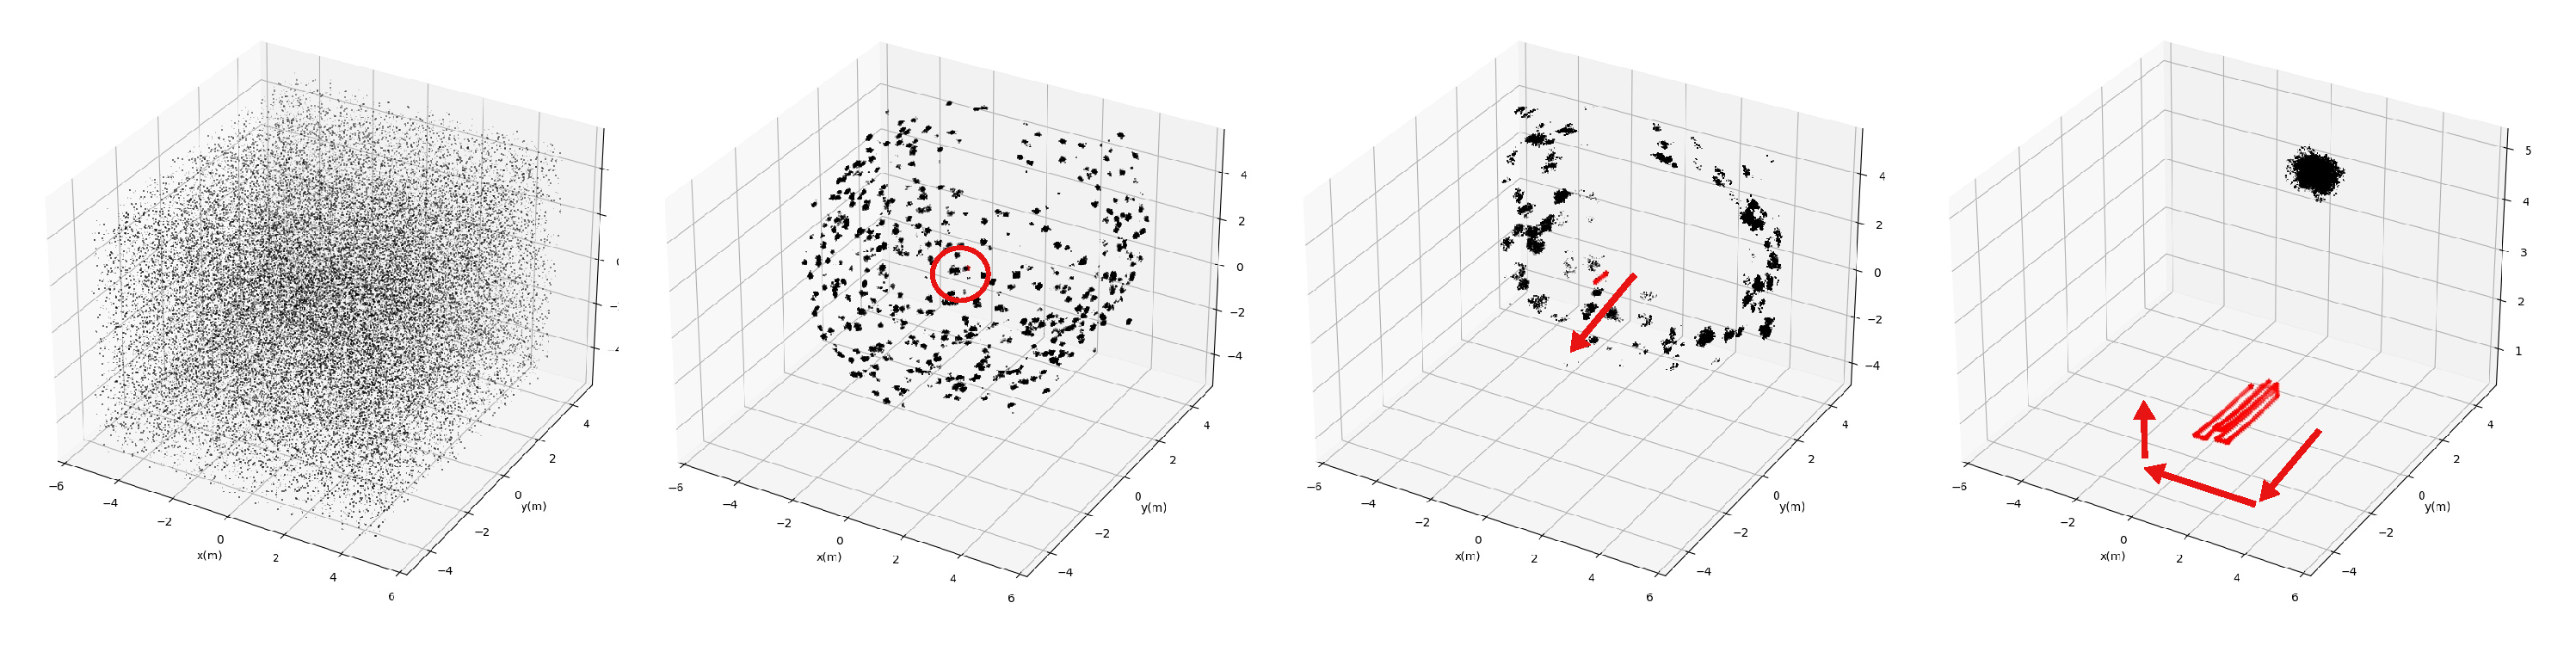
\includegraphics[width=1\linewidth]{img/monte_carlo}
	\caption{پالایش متوالی یک باور یکنواخت بر روی پارامترهای سینماتیکی از طریق الگوریتم مونت-کارلو}
	\label{fig:montecarlo}
\end{figure}

همانطور که در شکل 
\ref{fig:montecarlo}
نشان داده شده است، در ابتدا وقتی اطلاعاتی به فیلتر تزریق نمی‌شود، ذرات به طور یکنواخت در منطقه پخش می‌شوند(اولین نمودار از چپ). اما، همانطور که در شکل (نمودار دوم از چپ) نشان داده شده است، پس از کمی حرکت دادن دوربین در طول یک خط مستقیم، توزیع یکنواخت به یک پوسته کروی تبدیل می‌شود که تمامی مکان‌های ممکن برای مکان پولی را نشان می‌دهد و ضخامت آن عدم قطعیت بر طول اولیه کابل را نشان می‌دهد. به تدریج، با حرکت طولانی‌تر انتهای ربات و در امتداد جهت‌های دیگر، کره به یک حلقه تبدیل می‌شود همانطور که در شکل (نمودار سوم از چپ) نشان داده شده است. در نهایت به یک خوشه بیضوی از ذرات که مکان شناسایی شده نقطه پولی و عدم قطعیت مربوطه آن را نشان می‌دهد تبدیل می‌شود که در شکل (نمودار چهارم از چپ) نشان داده شده است.

\subsection{ترکیب بینایی-سینماتیک و استفاده از گراف عامل معرفی شده}
در این بخش، ما گراف عامل را که در بخش 
\ref{seq:factor_graph_for_rigid_cable}
 بیان شده است، پیاده‌سازی می‌کنیم تا پارامترهای مراحل قبل را با در نظر گرفتن تأثیر متقابل تمام حالت‌ها بهبود دهیم. ما این گراف عامل را با استفاده از کتابخانه GTSAM
\cite{dellaert2012factor}
 که یک حل‌کننده معروف در جامعه SLAM است و حالت‌های اجرای افق متحرک و افزایشی بسیار کارآمدی دارد، پیاده‌سازی می‌کنیم. گراف‌های عامل این گراف به صورت دستی در کلاس‌های C++ نوشته شده و به حل‌کننده این کتابخانه متصل شده‌است. 
 
\begin{table}[!t]
	\small
	\centering
	\caption{خطای مکان‌یابی با روش‌های مختلف (واحد متر)}
	\label{tab:calibration_results}
	\renewcommand{\arraystretch}{1.0} % Increase row spacing Me?
	\footnotesize
	\begin{tabular}{c|c|c|c}
		\toprule
		\rowcolor{gray!10}
		\hline
		\text{رشته} & \rl{خطای MSE سیتنماتیک مستقیم} & \rl{خطای MSE بینایی حرکتی} &  \rl{خطای MSE روش پیشنهادی}\\
		\midrule
		$01$ &  $0.036$ &  $0.05$  &   $0.029$ \\
		\hline
		$12$ &  $0.035$  &  $0.03$  &   $0.028$ \\
		\hline
		$\textbf{میانگین}$ &  $0.0355$ & $0.04$ & $0.0285$ \\
		\bottomrule
	\end{tabular}
\end{table}
 
 
مزایای ترکیب سینماتیک و حسگر بینایی در بهبود نتایج نقش موثری داشته است.جدول 
\ref{tab:calibration_results}
خلاصه‌ای از این نتیجه را در هر حالت ارائه می‌دهد. همانطور که انتظار می‌رود، دقت کلی با ترکیب این دو حالت بهبود می‌یابد. به ویژه برای رشته داده 01، ترکیب بینایی-سینماتیک به بهبود دقت 23 درصدی در مقایسه با سینماتیک مستقیم و 72 درصدی در مقایسه با بینایی حرکتی منجر می‌شود. این اعداد به ترتیب برای رشته داده 12 برابر با 25 درصد و 7 درصد است. بهبود عملکرد در رشته داده 01 بیشتر است، که با این واقعیت همخوانی دارد که انتهای ربات در این رشته داده حرکات پویاتری دارد و در نتیجه بینایی حرکتی در معرض تخریب بیشتری قرار می‌گیرد. از سوی دیگر، این حرکات پویا نوسانات بزرگی ایجاد می‌کنند که از حالت‌های سینماتیک قابل مشاهده نیستند و منجر به خطاهای نسبتاً بزرگی می‌شوند که در
\cite{allak2022kinematics}
نیز نشان داده شده است.







در ادامه، کاهش خطای پنجه ربات را پس از بهبود پارامترهای اولیه بررسی می‌کنیم. این خطا را به عنوان میانگین مربع خطا بین طول کابل محاسبه شده از معادله 
\ref{eq:cable_length_without_young_module}
 و مقادیر داده‌های انکودر از ربات تعریف می‌کنیم. ما از این خطا به عنوان یک معیار جانشین برای مکان‌های نقاط پولی استفاده می‌کنیم زیرا در پیاده‌سازی ما، قرقره‌ها در خارج از میدان دید سیستم ردیابی ما (سیستم داده‌های مرجع\footnote{\lr{Ground Truth (GT)}}
 ) قرار دارند و بنابراین مقادیر واقعی متناظر در نسخه فعلی مجموعه داده در دسترس نیستند. 
 
 \begin{figure}
 	\centering
 	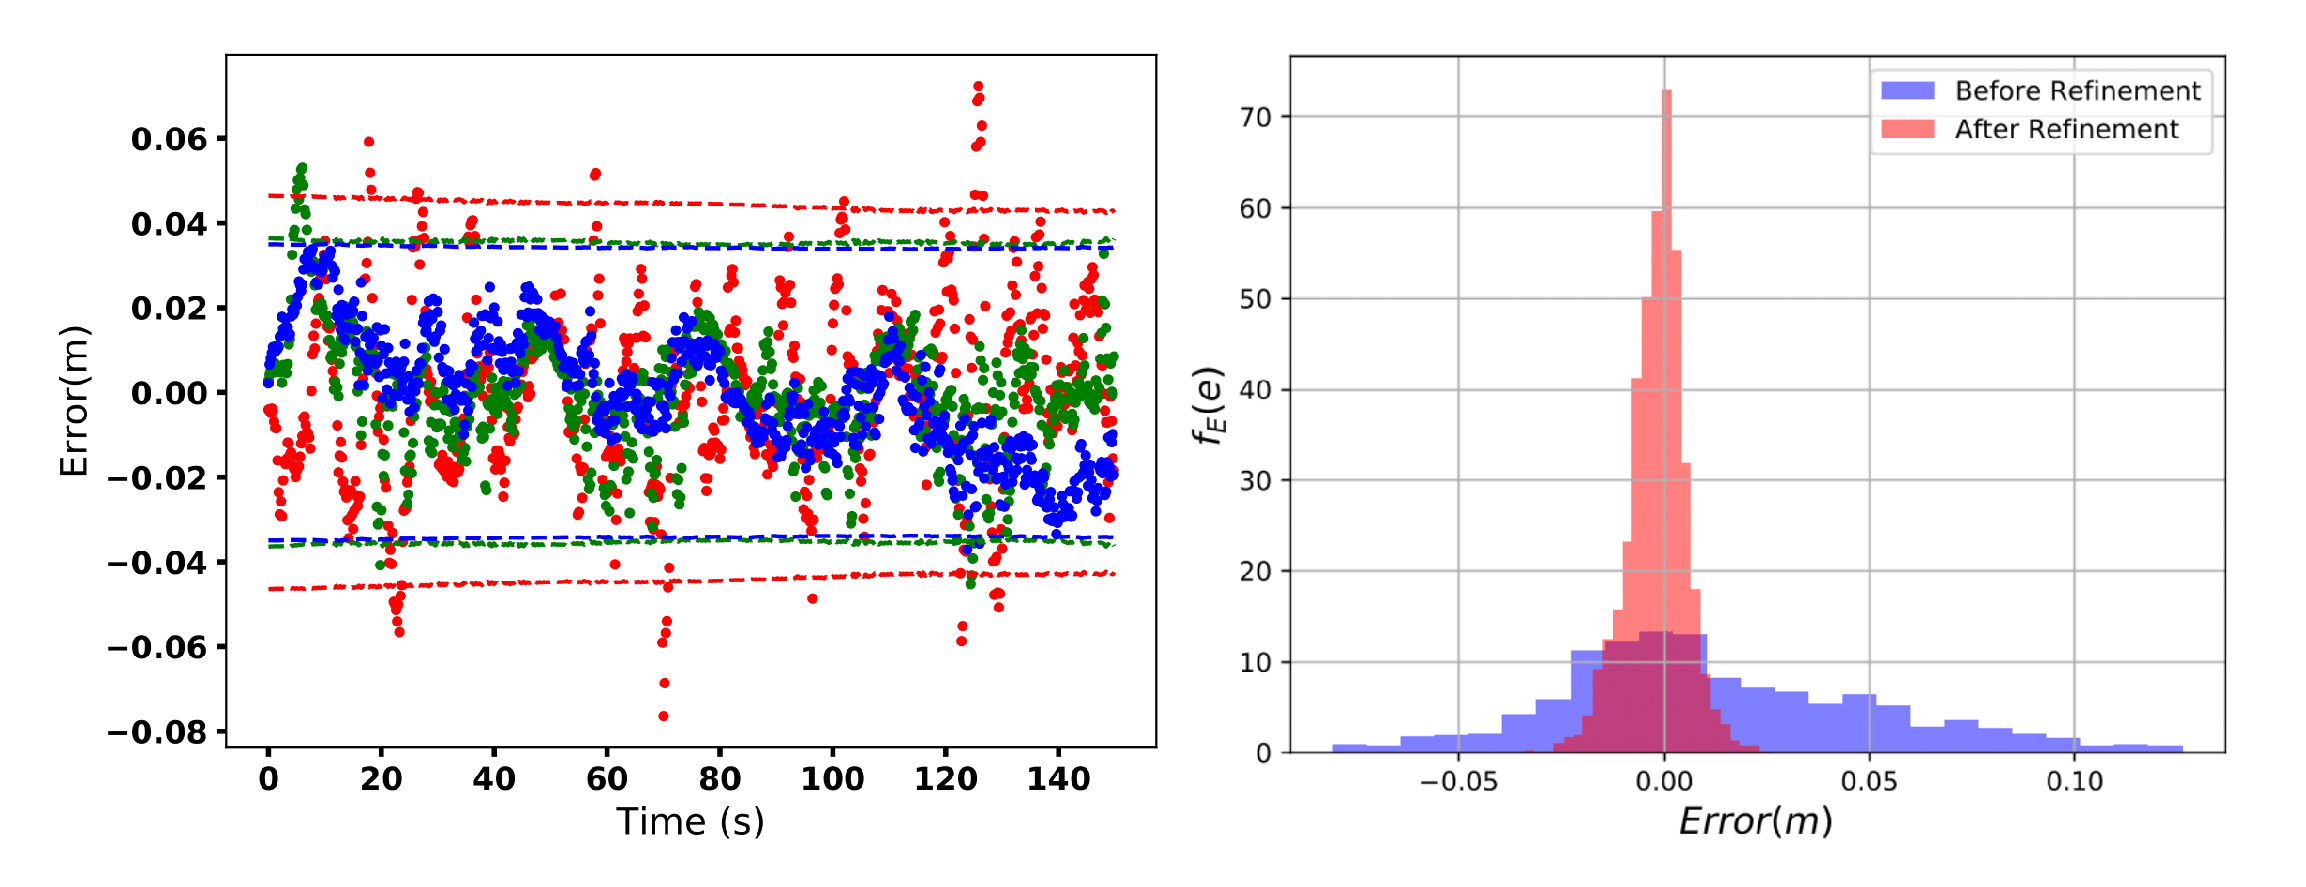
\includegraphics[width=0.9\linewidth]{img/calibration_result_rigid}
 	\caption{ راست: توزیع خطای پنجه قبل و بعد از بهبود پارامترها، چپ: خطای مکان‌یابی در دستگاه کارتزین}
 	\label{fig:calibrationresultrigid}
 \end{figure}
 
 شکل 
 \ref{fig:calibrationresultrigid}
 (نمودار سمت راست)
 توزیع خطای پنجه ربات را قبل و بعد از بهبود پارامترها نشان می‌دهد. همان‌طور که دیده می‌شود، میانگین و واریانس این خطا به طور قابل‌توجهی پس از بهبود کاهش یافته است. به طور خاص، برای رشته داده 01، مقدار خطا قبل از بهبود $0.043$ متر و پس از بهبود $0.0049$ متر است که نشان‌دهنده یک کاهش مرتبه‌ای در خطا است. این مقادیر برای رشته داده 12 به ترتیب $0.03$ متر قبل و $0.0053$ متر بعد از بهبود هستند. همچنین شکل 
  \ref{fig:calibrationresultrigid}
  (نمودار سمت چپ)
  نشان‌دهنده خطای مکان‌یابی پنجه ربات در دستگاه کارتزین در واحد متر می‌باشد. این خطا بیانگر اختلاف مقادیر مکان پنجه در سه جهت از حل گراف عامل نسبت به مقادیر داده‌های مرجع می‌باشد.

در نهایت، نتایج کیفی اجرای الگوریتم ما بر روی رشته داده 01 در شکل 
\ref{fig:trajectoryandpullyinrigidcable} 
نشان داده شده است. در این شکل، مسیر سیاه رنگ نمایانگر داده‌های مرجع و نقاط قرمز نشان‌دهنده مکان‌های اصلاح شده ربات توسط الگوریتم ما هستند. علاوه بر این، ستاره‌های آبی در شکل مکان‌های پولی قبل از بهبود و دایره‌های قرمز، آن‌ها را پس از بهینه‌سازی مشترک گراف عامل را نشان می‌دهند.

\begin{figure}
	\centering
	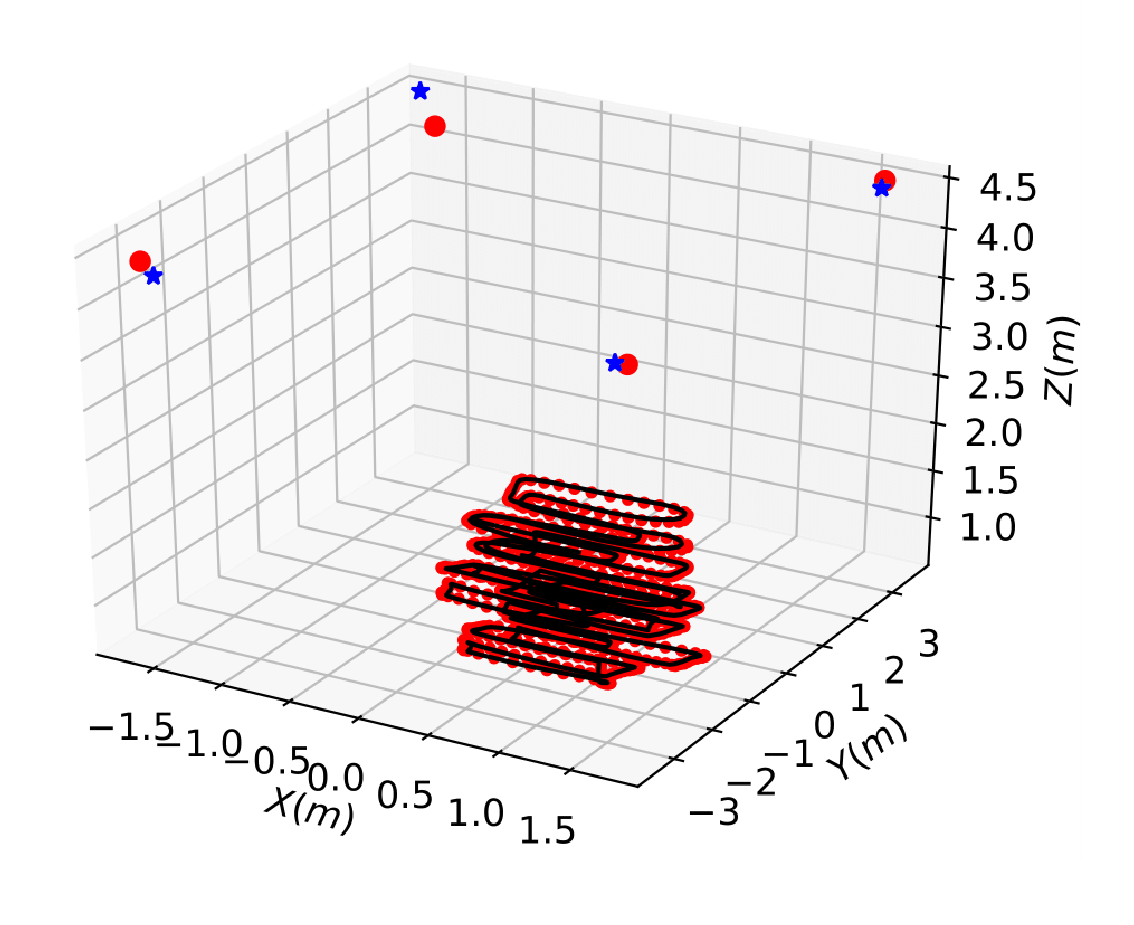
\includegraphics[width=0.5\linewidth]{img/trajectory_and_pully_in_rigid_cable}
	\caption{مسیر طی شده توسط ربات در کنار مکان اولیه و نهایی(بهبودیافته) پولی‌ها}
	\label{fig:trajectoryandpullyinrigidcable}
\end{figure}


\subsection{انتشار عدم قطعیت}
یکی از مزایای چارچوب پیشنهادی، توانایی آن در حفظ و در نظر گرفتن عدم قطعیت و نویز حسگر در طول فرآیند تخمین است. در پیاده‌سازی‌های ما، از مقادیر میانگین و ماتریس‌های کواریانس از برای راه‌اندازی الگوریتم با مقید کردن گراف عامل با استفاده از عامل‌های پیشین استفاده می‌کنیم. نتیجه این کار شباهت عدم قطعیت نهایی گراف عامل به توزیع خطای واقعی است.
ما این سازگاری را با تعیین درصد مقادیر خطا در محدوده‌های $\sigma$، $2\sigma$ و $3\sigma$ بررسی می‌کنیم.

 همانطور که در جدول 
\ref{tab:uncertainty_consistency}
 نشان داده شده است، تقریباً 60 درصد از خطاها در محدوده $\sigma$، 90 درصد در محدوده $2\sigma$ و تقریباً 98 درصد در محدوده $3\sigma$ قرار دارند.
نتایج جدول 
\ref{tab:uncertainty_consistency}
 نزدیک به محدوده‌های تئوریکی $\sigma$ هستند اما نشان‌دهنده یک پاسخ کمی بیش از حد مطمئن است. باید توجه داشت که سازگاری به شدت به مدل‌های حسگر مفروض و همچنین عدم قطعیت بینایی حرکتی تجربی برای الگوریتم SVO وابسته است. ما بررسی دقیق‌تر سازگاری عدم قطعیت را به کارهای آینده موکول می‌کنیم.

\begin{table}[!t]
	\small
	\centering
	\caption{سازگاری آماری عدم قطعیت‌های تخمین زده شده}
	\label{tab:uncertainty_consistency}
	\renewcommand{\arraystretch}{1.0} % Increase row spacing Me?
	\footnotesize
	\begin{tabular}{c|c|c|c}
		\toprule
		\rowcolor{gray!10}
		\hline
		\text{محور} & \rl{$\sigma$} & \rl{$2\sigma$} & \rl{$3\sigma$} \\
		\midrule
		$x$ &  $53\%$ &  $82\%$  &   $95\%$ \\
		\hline
		$y$ &  $71\%$  &  $92\%$  &   $97\%$ \\
		\hline
		$z$ &  $51\%$ & $88\%$ & $99\%$ \\
		\bottomrule
	\end{tabular}
\end{table}


\section{بحث و گفت‌وگو}
روش پیشنهادی در این فصل یک دیدگاه منعطف و یکپارچه در مورد کالیبراسیون و برآورد حالت برای ربات‌های کابلی صلب ارائه می‌دهد. این یکپارچگی در جامعه SLAM به شکل اجرای موازی تنظیم مجموعه\footnote{\lr{Boundle Adjustment (BA)}}
 و ردیابی دوربین\footnote{\lr{camera tracking}}
 به خوبی شناخته شده است. به ویژه برای عملکرد بلادرنگ\footnote{\lr{real time}}
 ، مرحله گراف عامل الگوریتم ما ممکن است به صورت افق متحرک حل شود و حالت‌های قدیمی به فاکتورهای پیشین حاشیه‌سازی شوند. از سوی دیگر، کالیبراسیون اولیه ممکن است بدون محدودیت بلادرنگ و با استفاده از اجرای دسته‌ای گراف روی رشته داده طولانی‌تری انجام شود.

پیاده‌سازی فعلی ما در Python روی یک لپ‌تاپ شخصی با پردازنده Intel Core-i7 و 16 گیگابایت RAM کمتر از یک دقیقه برای هر کابل زمان می‌برد تا روش ابتدایی مونت-کارلو را اجرا کند (برای 750 وضعیت دوربین و 5000 ذره) و حدود 30 ثانیه زمان برای بهبود آن‌ها توسط گراف عامل. حالت‌های اجرای افق متحرک حل‌کننده‌های بسیار کارآمد برای گراف‌های عامل مانند 
\cite{dellaert2012factor} و \cite{martiros2022symforce}
 از جامعه SLAM می‌توانند فرکانس برآورد مکان را به نرخ فریم دوربین افزایش دهند که برای بیشتر کنترل‌کننده‌های حلقه خارجی مناسب است. ما بررسی بیشتر عملکرد بلادرنگ الگوریتم خود را به کارهای آینده موکول می‌کنیم.

یکی دیگر از جنبه‌های مهم الگوریتم پیشنهادی، ماژولار بودن آن است. به ویژه، این فرمول‌بندی اجازه می‌دهد تا دیگر حالت‌ها از جمله اما نه محدود به IMU، UWB و حسگرهای سیستم به راحتی به گراف عامل اضافه شوند. علاوه بر این، اندازه‌گیری‌های شبه‌هندسی مانند هم‌سطحی نقاط پولی (به عنوان مثال دو پولی در همان دیوار) یا فاصله بین مکان‌های پولی (قابل اندازه‌گیری با استفاده از ابزارهای اندازه‌گیری کم‌هزینه) به راحتی در مسئله گنجانده می‌شوند که به طور قابل‌توجهی به دقت کلی تخمین کمک می‌کند.

در نهایت، سیستم پیشنهادی ممکن است به طور مستقیم برای کالیبراسیون سیستم‌های مکان‌یابی UWB استفاده شود. در این سیستم‌ها، مدل اندازه‌گیری فاصله بین تگ و انکرها دقیقاً با مدل کابل صلب در نظر گرفته شده در این فصل یکسان است. ما قصد داریم این موضوع را به عنوان کارهای آینده بیشتر بررسی کنیم.


\section{نتیجه‌گیری}

در این فصل، ما پیشنهاد دادیم که از ترکیب داده‌های دوربین و حسگرهای سینماتیکی موجود در ربات به منظور ایجاد یک چارچوب تلفیق آماری برای کالیبراسیون و مکان‌یابی ربات‌های کابلی استفاده شود. این هدف با فرمول‌بندی یک الگوریتم مونت-کارلو که نمایشی از مسئله در ساختار گراف عامل را مقداردهی اولیه می‌کند، محقق شد. رویکرد ما نیازی به استفاده از نشانگرهای خاص نداشت و به جای آن، از راه‌حل‌های عمومی‌تر SLAM برای تخمین حرکت پنجه ربات استفاده کرد. از طریق آزمایش‌های عملی با استفاده از یک مجموعه داده واقعی که توسط ربات \lr{ARAS-CAM} ضبط شده بود، ما عملکرد این رویکرد را ارزیابی کردیم و نشان دادیم که تلفیق داده‌ها باعث افزایش دقت شده و همچنین امکان شناسایی پارامترهای سینماتیکی بدون نیاز به فرضیات اولیه قوی را فراهم می‌کند. 
